\chapter{Details}\label{chap:details}
\section{States and Transitions}\label{sec:search}
In the following graphs, the light blue (cyan) traces represent ``nodes that were considered'' along the way to a solution, and the red trace represents the ``final solution''.  The number of nodes popped from the stack or queue during each algorithm is noted, along with cost or distance of the path.

\subsection{Depth First Search}
The \texttt{depth first} search was the wildest of the bunch (see Figure ~\ref{fig:df}), and clearly not optimal: its ``solution'' goes all over the map and finally settles on a path that winds back and forth across half of the map.  Nodes popped: 2,411.  Distance of the path: 12,154 meters.

\begin{figure}\label{fig:df}
\begin{center}\centering
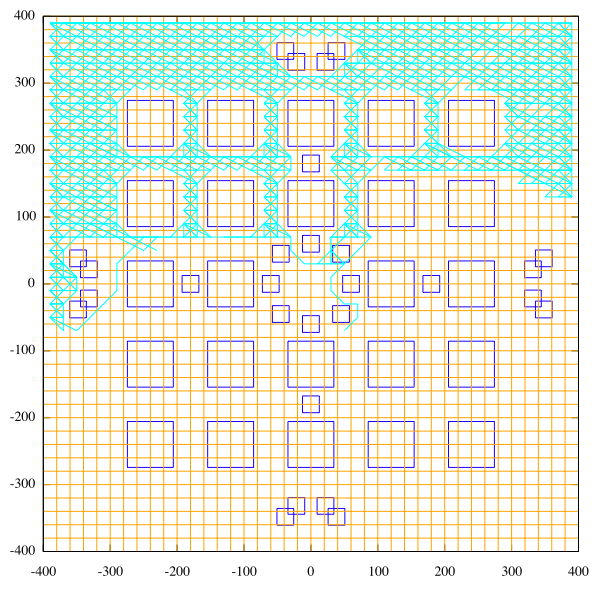
\includegraphics[width=\textwidth]{df1.png}
\caption{Depth first grows}
\end{center}
\end{figure}

\begin{figure}
\begin{center}\centering
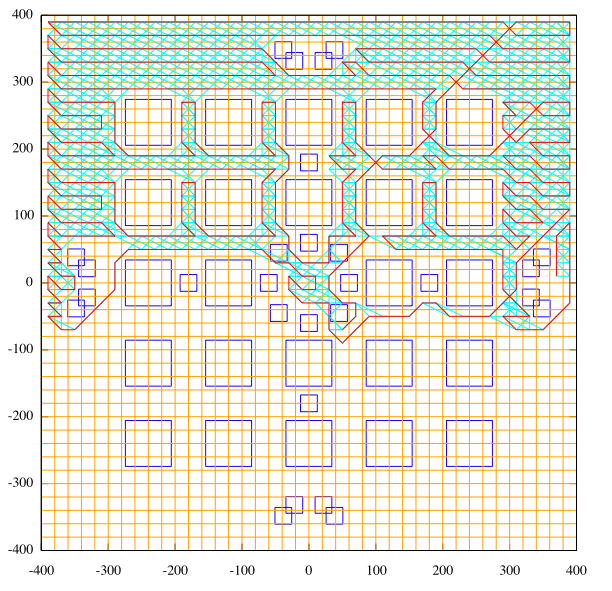
\includegraphics[width=\textwidth]{df2.png}
\caption{Depth first finds a solution}
\end{center}
\end{figure}

\subsection{Breadth First Search}
The \texttt{breadth first} search was one of our cleanest solutions, even though it takes the most memory.  In the Figure ~\ref{fig:bf} the search grows outward from a central location, and then (in the following figure) finds an optimal solution.  Nodes popped: 7,922.  Distance of the path: 1,010 meters.

\begin{figure}\label{fig:bf}
\begin{minipage}[b]{0.3\linewidth} % A minipage that covers half the page
\centering
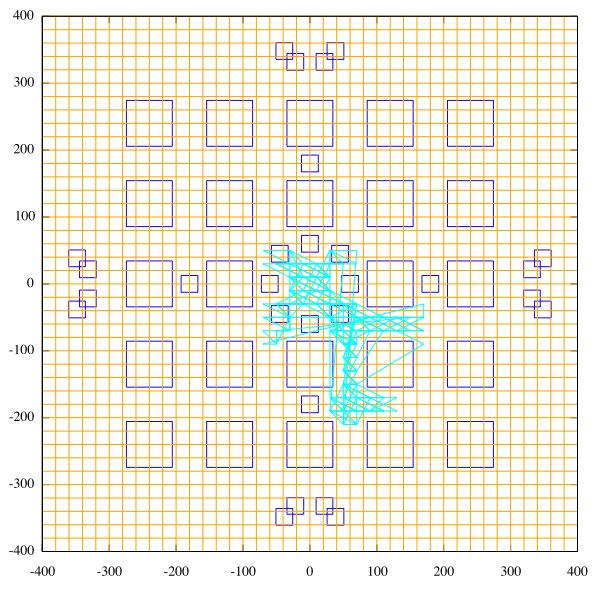
\includegraphics[width=0.9\linewidth]{bf1.png}
\end{minipage}
\hspace{0.5cm} % To get a little bit of space between the figures
\begin{minipage}[b]{0.3\linewidth}
\centering
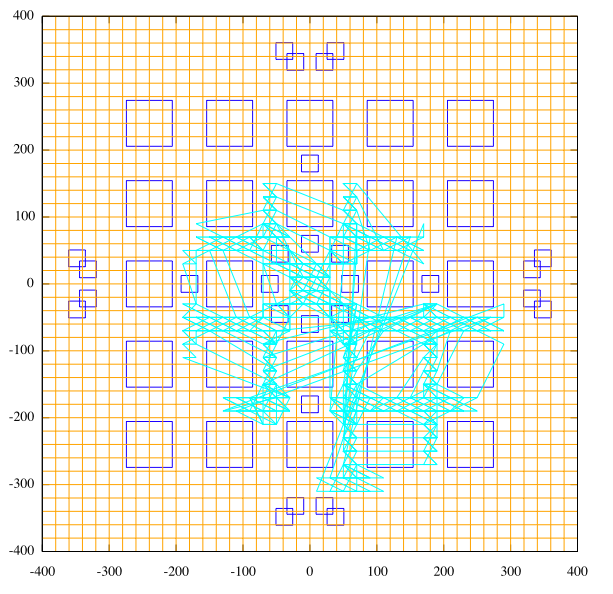
\includegraphics[width=0.9\linewidth]{bf2.png}
\end{minipage}
\hspace{0.5cm} % To get a little bit of space between the figures
\begin{minipage}[b]{0.3\linewidth}
\centering
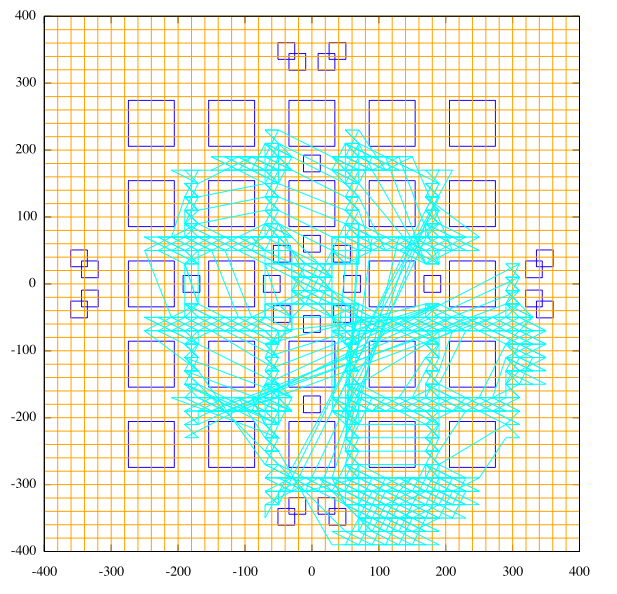
\includegraphics[width=0.9\linewidth]{bf3.png}
\end{minipage}
\caption{Breadth first grows}
\end{figure}

\begin{figure}\label{fig:bfsol}
\begin{center}\centering
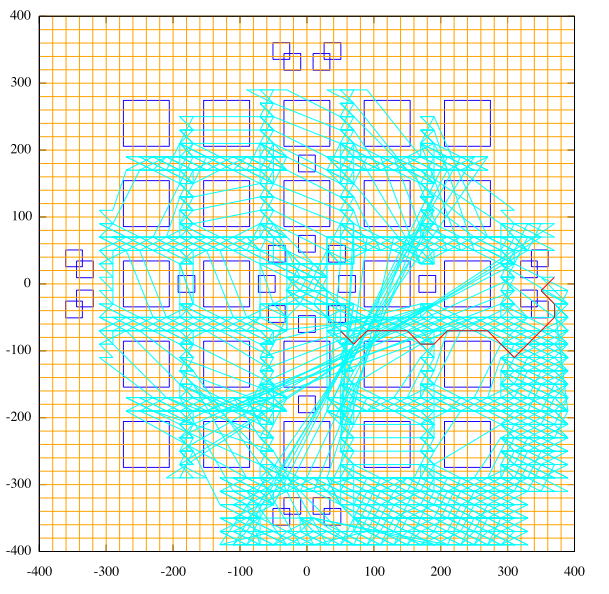
\includegraphics[width=0.8\textwidth]{bf4.png}
\caption{Breadth first finds a solution}
\end{center}
\end{figure}

\subsection{Iterative Deepening Search}
The \texttt{iterative deepening} search was the most time-intensive of the group, and in order to complete it we had to significantly reduce the search space.  In addition---unlike other experiments---we moved the flag and the tank close together so that it would only have to search within a radius of 5 squares for the solution.  Our Ruby implementation of \texttt{iterative deepening} would not run past 10 iterations due to time constraints.  Nodes popped: 215.  Distance of the path: 419 meters.

\begin{figure}
\begin{center}\centering
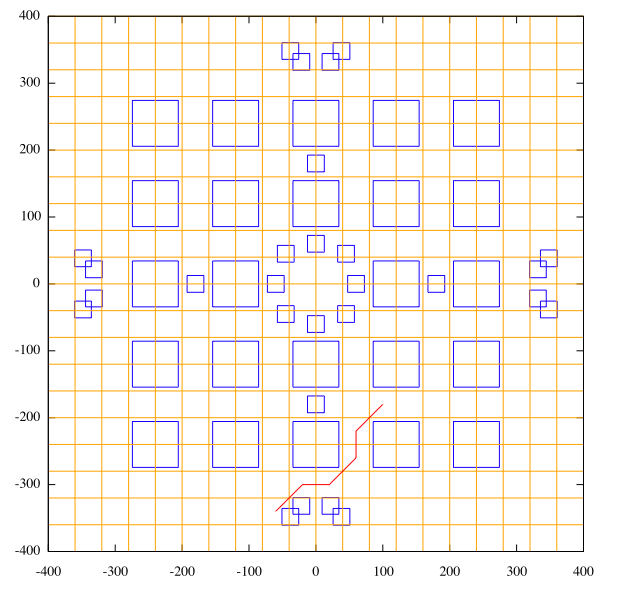
\includegraphics[width=\textwidth]{id1.png}
\caption{Iterative deepening (The start point and the flag have been moved close together in order to find a path in a reasonable amount of time)}
\end{center}
\end{figure}

\subsection{Greedy Best First Search}
The \texttt{greedy best first} algorithm was by far the fastest algorithm that we experimented with.  Its solution, while not optimal, is also one of the best.  See Figure ~\ref{fig:gbf}.  Nodes popped: 114.  Distance of the path: 1,485 meters.

\begin{figure}\label{fig:gbf}
\begin{center}\centering
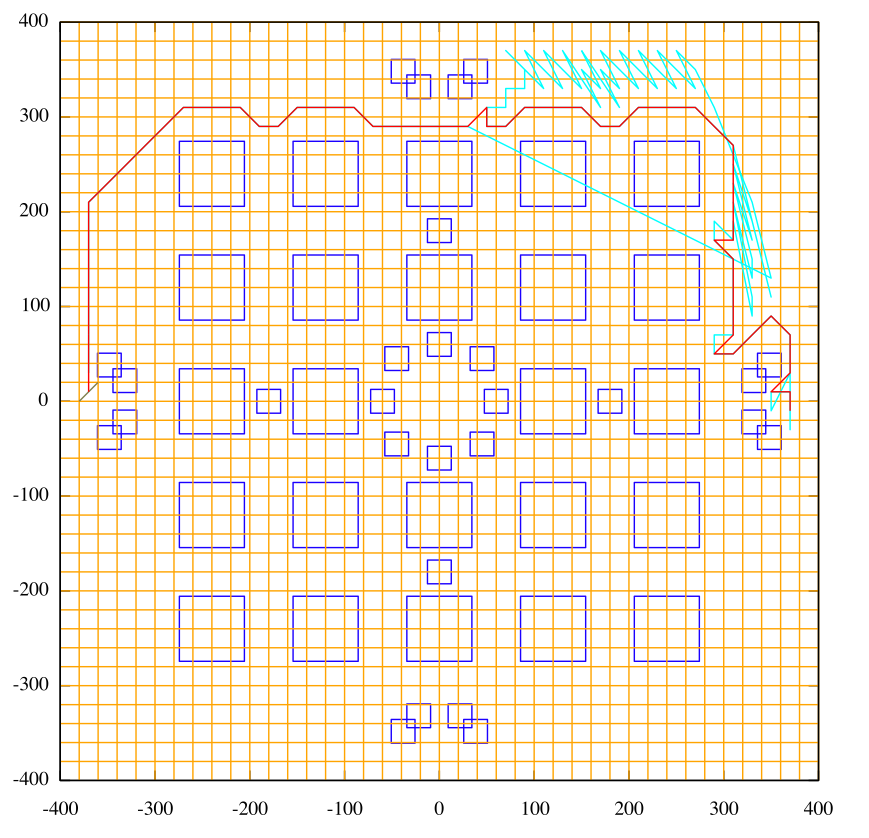
\includegraphics[width=\textwidth]{gbf.png}
\caption{Greedy best first solution}
\end{center}
\end{figure}


\subsection{$A^*$ Search}
The $A^*$ solution is clean and direct---it seems to follow the most accurate path through the center and then to the destination.  It is also interesting to see how it first considered a route that skirts around the main obstacles by heading `south', but then settles on a path through the middle.  See Figure ~\ref{fig:astar}.  Nodes popped: 190.  Distance of the path: 946 meters.
\par
In addition to a simple $A^*$ search, we also placed a tank in the middle of the game board so as to be able to observe an effect on the search path outcome.  When we placed a tank in the way of the search, the algorithm chose a path that popped 44 nodes and had a distance of 934 meters.

\begin{figure}\label{fig:astar}
\begin{center}\centering
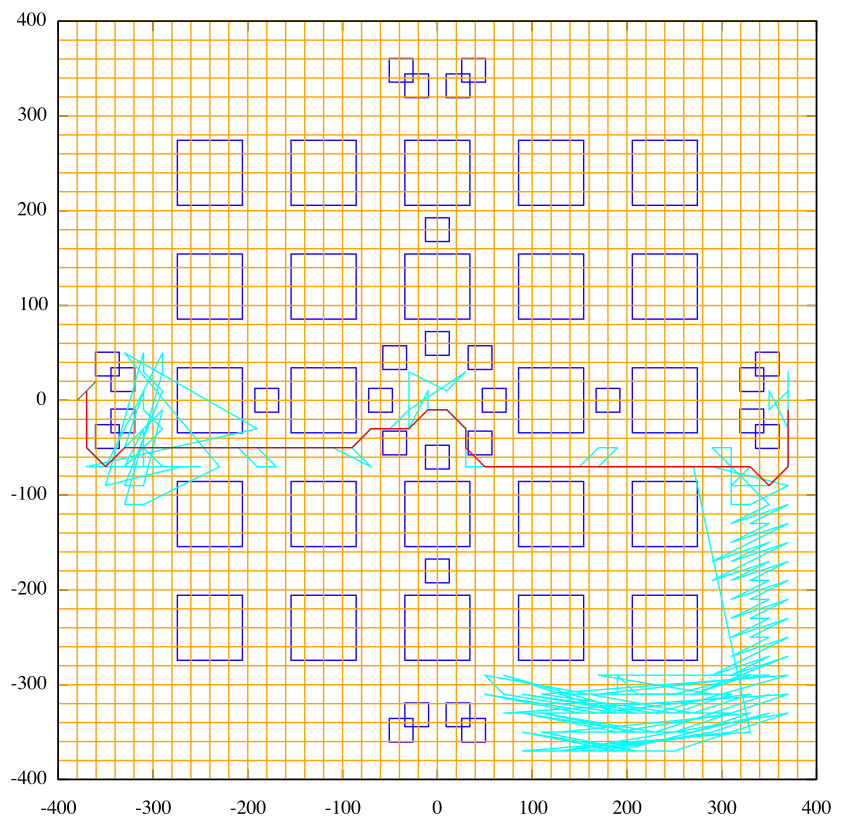
\includegraphics[width=\textwidth]{astar.png}
\caption{$A^*$ solution}
\end{center}
\end{figure}

\section{Adventures in Heuristics}
The obvious heuristic to use on a full-observable map is the straight-line heuristic.  The straight-line is admissible which guarantees us an optimal result.  We didn't bother changing our heuristic (other than to enforce penalties) for the rest of the lab until we started this report.  The consequence of not changing our heuristic until asked to do so is that our alternate heuristics are somewhat contrived, but did provide interesting results.
\par
The first alternate heuristic we tried was a polynomial that took the square of the straight-line distance and added 183 (see Figure ~\ref{fig:poly}).  We hoped that because this heuristic is not admissible that we would get a suboptimal answer---and we did.
\begin{figure}\label{fig:poly}
\begin{center}
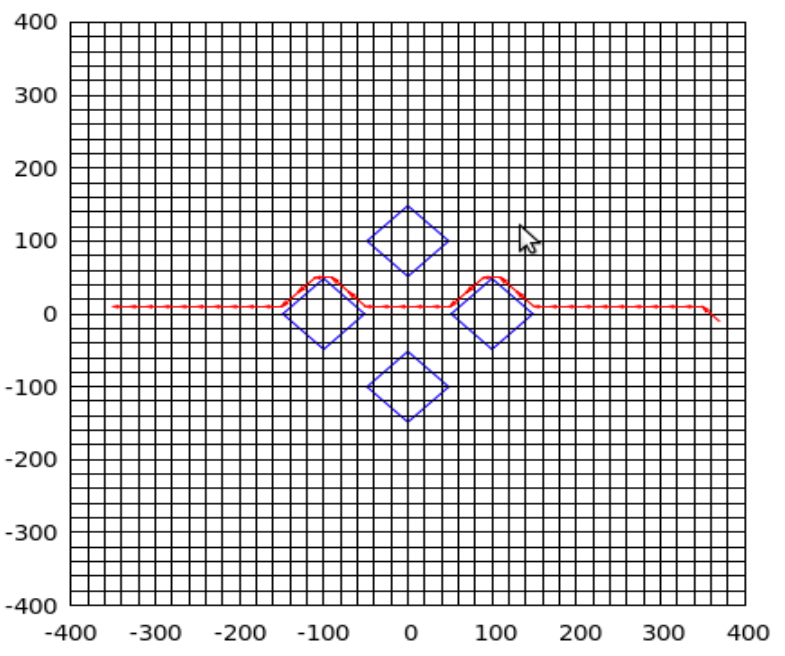
\includegraphics[width=\textwidth]{heur1.png}
\caption{Polynomial heuristic $d^2 + 183$}
\end{center}
\end{figure}
The solution looks very much like a \texttt{greedy best first} solution because the heuristic diminishes as a square the closer we get to the goal so that the path-cost is never a competitive factor with the heuristic.  The $A^*$ algorithm ended up choosing the same solution as the \texttt{greedy best first} when using this heuristic.  In the end this mean that we considered 38 nodes, used 37 of them in the final solution and traversed a total of 814.5 meters.
\par
The next alternate heuristic we tried (see Figure ~\ref{fig:circ}) was to find the circular arc distance between our current node and the goal.  This ends up being a multiplicative constants of $\pi$.  I assumed that multiplying everything by $\pi$ would have a null effect since it would be a uniform penalty on all nodes, but in fact it did change the solution quite a bit.
\begin{figure}\label{fig:circ}
\begin{center}
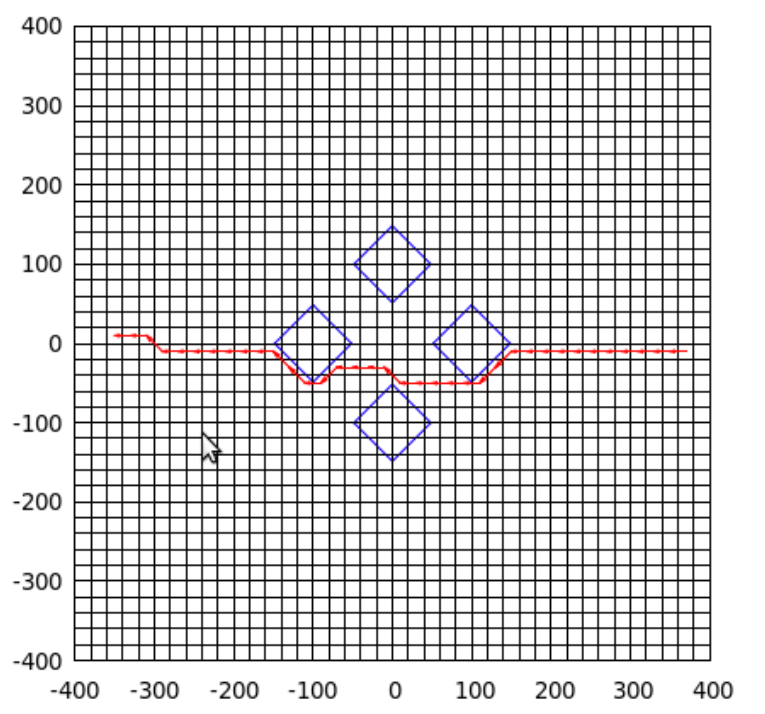
\includegraphics[width=\textwidth]{heur2.png}
\caption{Circular arc distance heuristic}
\end{center}
\end{figure}
This solution was sub-optimal and took the `southern road' below the obstacles rather than passing above them.  This solution evaluated 38 nodes and used 37 of them in the solution which was on-par with the polynomial heuristic.  The total distance traveled was 797.9 meters which is less than the polynomial heuristic above.  The reason that this multiplicative constant ended up affect our final solution is that it affects our heuristic, but not our cost path.  So our total cost for each node was an imbalanced summation of the heuristic and the path cost.
\par
Finally using our straight-line heuristic we came up with an optimal solution that took a lot longer to compute.  See Figure ~\ref{fig:straight}.

\begin{figure}\label{fig:straight}
\begin{center}
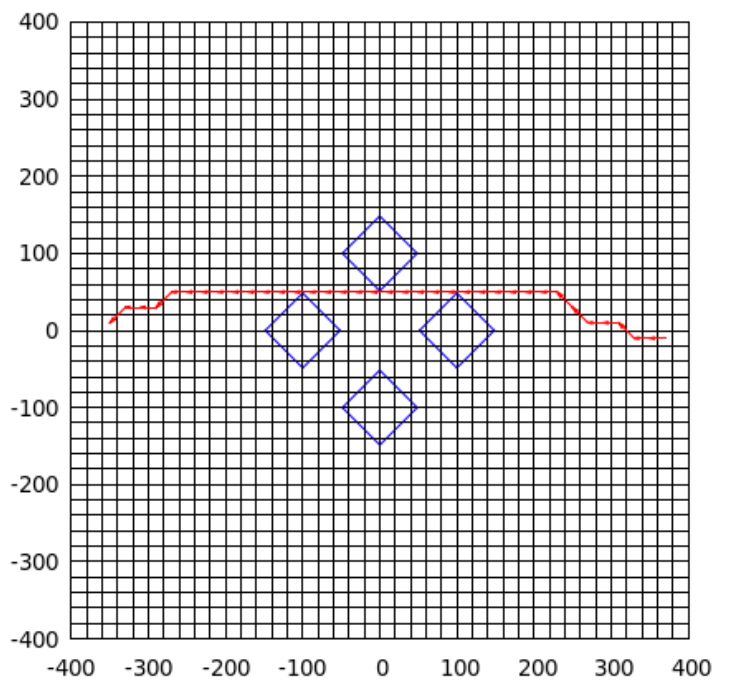
\includegraphics[width=\textwidth]{heur3.png}
\caption{Straight-line distance heuristic}
\end{center}
\end{figure}


\section{Path Following and Potential Fields}
While developing our search algorithms in the last lab we realized that doing full $A*$ searching was not going to be possible in ruby if our discretization was too granular. To alleviate this problem Duane Johnson developed a small library written in C which acted as a module to the rest of our code.  We also simplified the representation of the discretized map for the algorithm to search through.  With these changes we were able to search through maps of 80x80 in approximately 1/10 of a second.  This was fast enough and granular enough for the purpose of finding our way through a maze and deploying a decoy-sniper tactic.
\par
When it came time to follow the solution path returned by Duane's $A*$ module the immediate thought was to use potential fields along the length of the path.  The potential fields code developed in the first lab already had a PD controller which would suggest velocity and angular velocity based on the current position and angle of the tank.  As the lab progressed we optimized this algorithm to actually look as far ahead as the line segments are parallel so that when driving in a straight line we don't spend much time re-evaluating the path.
\par
In addition to the path following optimizations we also 'tuned' the relative strength of the fields and their radii so that as we approach the next Potential Field the system will move it to the next location before our arrival.  This helped to avoid uneccesary 'braking' and turning.

\section{Tests with Another Group}
\subsection{Our Tests}
All of our tests were run on the default BZFlag map with 24 large obstacles and 28 small.  In most cases, our team was the `green' team on the `east' side of the game area and was attempting to search out the `red' team on the `west' side of the game area.  In the case of \texttt{breadth first} search, the tank started somewhere near the middle of the game area, and targetted a flag on the `east' side.
\par
For each algorithm, the `nodes popped' and path distances were recorded in section ~\ref{sec:search}.  The numbers seem reasonable except in the case of our \texttt{iterative deepening} search, where the nodes popped are significantly lower than expected.  This is in part because our algorithm was so slow that we needed to give it a little boost by putting the tank close to the goal---very close, in fact.  Thus, our measurements in this particular case are not comparable with the other algorithm measurements.

\subsection{Dave Brinton et. al.}
We helped test with Dave Brinton et. al.  Their procedure went smoothly, and in particular, their gnuplot maps were especially good---their maps branched at each cell as it checked successors, showing a line from each cell to its successor cells.  This animation made it very clear what their algorithms were doing.
\par

\begin{itemize}
    \item \texttt{breadth first}	Nodes popped: 1,098, Distance: 1,018 m.
    \item \texttt{depth first}	Nodes popped: 292, Distance: 6,368 m.
    \item \texttt{iterative deepening}	Nodes popped: 3,074,227, Distance: 504 m.
    \item \texttt{greedy best first}	Nodes popped: 54, Distance: 1,049 m.
    \item $A^*$	Nodes popped: 1,028, Distance: 1,047 m.
    \item $A^*$ (with tank) Nodes popped: 1,023, Distance: 1,047 m.
\end{itemize}

For each of the search tests above, we chose the default map, except in the cases of \texttt{depth first} and \texttt{iterative deepening}, where the ``Four Ls'' map was chosen.







